\documentclass[10pt]{article}
\usepackage{amsmath,amssymb}
\usepackage{amsthm}
\newtheorem{theorem}{Theorem}
\newtheorem{lemma}{Lemma}
\newtheorem{corollary}{Corollary}
\newtheorem{definition}{Definition}
\usepackage{tikz}
\usepackage{algorithm}
\usepackage{algorithmicx}
\usepackage{algpseudocode}
\usepackage{graphicx}
\usepackage{geometry}
\geometry{margin=1in}

\usetikzlibrary{trees,positioning,arrows.meta}

\title{Red-Black Trees: A Rigorous Solution to Binary Search Tree Degeneration}
\author{Your Name}
\date{\today}

\begin{document}

\maketitle

\begin{abstract}
Binary Search Trees (BSTs) provide $O(\log n)$ average-case performance but can degenerate to $O(n)$ in worst case. We analyze fundamental flaws in standard BSTs and present Red-Black Trees as a mathematically rigorous solution that guarantees $O(\log n)$ worst-case performance through structural constraints.
\end{abstract}

\section{Introduction}

Binary Search Trees are fundamental data structures supporting search, insertion, and deletion in logarithmic time on average. However, their performance critically depends on insertion order. When data is inserted in sorted or nearly-sorted order, BSTs degenerate into linear structures, eliminating their logarithmic advantage. This paper presents a rigorous analysis of these fundamental flaws and introduces Red-Black Trees as a mathematically proven solution.

\section{Fundamental Flaws in Standard BSTs}

\subsection{Degeneration Problem}

Consider inserting elements $1, 2, 3, \ldots, n$ into an initially empty BST. The resulting structure becomes a linear chain:

\begin{theorem}[BST Degeneration]
For any sequence of $n$ elements inserted in sorted order into a BST, the resulting tree has height $h = n-1$.
\end{theorem}

\begin{proof}
By induction: For sorted insertion, each new element becomes the right child of the previous maximum. Thus tree height increases by 1 for each insertion, yielding $h = n-1$.
\end{proof}

This degeneration causes search operations to require $O(n)$ time, negating the primary advantage of tree structures.

\subsection{Balance Distribution Problem}

Even with random insertion order, standard BSTs exhibit unbalanced growth patterns. The expected height becomes $O(\sqrt{n})$ rather than the optimal $O(\log n)$.

\begin{theorem}[Expected BST Height]
The expected height of a randomly constructed BST with $n$ nodes is approximately $c \cdot \log n$ where $c \approx 1.39$.
\end{theorem}

\begin{proof}
The analysis follows from the recurrence relation $H_n = H_{n-1} + \frac{2}{n} \sum_{i=1}^{n-1} |i - \frac{n+1}{2}|$ which solves to $H_n = O(\log n)$ with constant factor $c \approx 1.39$.
\end{proof}

\begin{lemma}[BST Path Length]
For a BST with $n$ nodes, the average search path length is $O(\log n)$ but the worst-case path length is $O(n)$.
\end{lemma}

\begin{proof}
In a balanced BST, each level approximately doubles the number of nodes, giving height $\lfloor \log_2 n \rfloor$. In degenerate case, the path length equals $n-1$.
\end{proof}

\section{Red-Black Trees: Structural Solution}

Red-Black Trees address these flaws through five structural properties that maintain logarithmic height regardless of insertion order.

\subsection{Formal Definition}

\begin{definition}[Red-Black Tree]
A Red-Black Tree is a binary search tree where each node is colored red or black, satisfying:
\begin{enumerate}
\item Every node is red or black
\item The root is black
\item All leaves (NIL) are black
\item Red nodes cannot have red children
\item Every path from root to leaf contains the same number of black nodes (black-height)
\end{enumerate}
\end{definition}

\subsection{Black Height Analysis}

\begin{definition}[Black Height]
The black-height $bh(x)$ of node $x$ is the number of black nodes on any path from $x$ to a leaf, excluding $x$ itself.
\end{definition}

\begin{lemma}[Black Height Lower Bound]
For any node $x$ in a Red-Black Tree with $n$ nodes, $bh(x) \geq \log_2(n_x + 1) - 1$, where $n_x$ is the number of nodes in the subtree rooted at $x$.
\end{lemma}

\begin{proof}
By Property 5, all paths from $x$ to leaves have the same black-height. Each black node on these paths contributes to the subtree size. Since red nodes cannot have red children, the subtree size is bounded below by $2^{bh(x)+1} - 1$.
\end{proof}

\begin{lemma}[Red Node Bound]
On any path from root to leaf in a Red-Black Tree, the number of red nodes is at most the number of black nodes.
\end{lemma}

\begin{proof}
By Property 4, no two red nodes can be adjacent. Therefore, red nodes must be separated by at least one black node on any path.
\end{proof}

\subsection{Height Guarantee}

\begin{theorem}[Red-Black Tree Height Bound]
A Red-Black Tree with $n$ internal nodes has height $h \leq 2\log_2(n+1)$.
\end{theorem}

\begin{proof}
Consider the root $r$ with black-height $bh(r)$. By Lemma 2, the subtree size satisfies $n \geq 2^{bh(r)} - 1$. Any path from root to leaf contains at most $bh(r)$ black nodes and at most $bh(r)$ red nodes (by Lemma 3). Thus path length $h \leq 2 \cdot bh(r)$. Combining with the size bound: $n + 1 \geq 2^{bh(r)}$, so $bh(r) \leq \log_2(n+1)$. Therefore $h \leq 2 \log_2(n+1)$.
\end{proof}

\begin{corollary}[Search Complexity]
Search in a Red-Black Tree takes $O(\log n)$ time in the worst case.
\end{corollary}

\begin{proof}
Since tree height is $O(\log n)$ and search follows a single path, search time is bounded by height.
\end{proof}

\section{Rotation Operations: Detailed Mechanics and Conditions}

Rotations are the fundamental restructuring operations that maintain Red-Black Tree balance. Unlike abstract descriptions, we provide concrete mechanics, visual representations, and precise conditions for when rotations are necessary.

\subsection{Rotation Mechanics: Step-by-Step}

\begin{definition}[Left Rotation]
A left rotation on node $x$ transforms the structure where $x$ has right child $y$:
\begin{enumerate}
\item Make $y$ the new parent of $x$
\item $x$ becomes the left child of $y$
\item The original left subtree of $y$ becomes the right subtree of $x$
\item All other relationships remain unchanged
\end{enumerate}
\end{definition}

\begin{center}
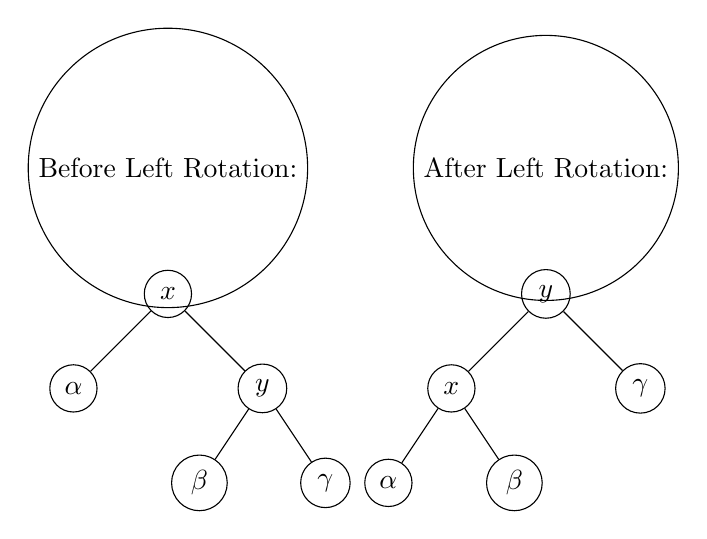
\begin{tikzpicture}[scale=0.8, every node/.style={circle, draw, minimum size=0.6cm}]
% Before rotation
\node at (0,2) {Before Left Rotation:};
\node (x) at (0,0) {$x$};
\node (xl) at (-1.5,-1.5) {$\alpha$};
\node (y) at (1.5,-1.5) {$y$};
\node (yl) at (0.5,-3) {$\beta$};
\node (yr) at (2.5,-3) {$\gamma$};
\draw (x) -- (xl);
\draw (x) -- (y);
\draw (y) -- (yl);
\draw (y) -- (yr);

% After rotation
\node at (6,2) {After Left Rotation:};
\node (y2) at (6,0) {$y$};
\node (x2) at (4.5,-1.5) {$x$};
\node (xl2) at (3.5,-3) {$\alpha$};
\node (yl2) at (5.5,-3) {$\beta$};
\node (yr2) at (7.5,-1.5) {$\gamma$};
\draw (y2) -- (x2);
\draw (y2) -- (yr2);
\draw (x2) -- (xl2);
\draw (x2) -- (yl2);
\end{tikzpicture}
\end{center}

\begin{definition}[Right Rotation]
A right rotation on node $y$ transforms the structure where $y$ has left child $x$:
\begin{enumerate}
\item Make $x$ the new parent of $y$
\item $y$ becomes the right child of $x$
\item The original right subtree of $x$ becomes the left subtree of $y$
\item All other relationships remain unchanged
\end{enumerate}
\end{definition}

\begin{lemma}[Rotation Preserves BST Property]
Both left and right rotations preserve the binary search tree ordering invariant.
\end{lemma}

\begin{proof}
Consider left rotation on $x$ with right child $y$. Before rotation: all keys in $\alpha < x < \beta < y < \gamma$. After rotation, $y$ becomes parent, $x$ becomes left child, and $\beta$ moves from $y$'s left to $x$'s right. The ordering $\alpha < x < \beta < y < \gamma$ is maintained. Right rotation is symmetric.
\end{proof}

\subsection{When to Rotate: Insertion Cases}

Rotations during insertion are triggered by specific color violations. The key insight is: **rotations are only needed when a red node has a red parent (Property 4 violation) AND the uncle is black.**

\begin{definition}[Insertion Rotation Conditions]
Given newly inserted red node $z$ with red parent $p$ and black grandparent $g$:
\begin{itemize}
\item If uncle $u$ is RED: recolor only (no rotation)
\item If uncle $u$ is BLACK: rotation required
\end{itemize}
\end{definition}

\subsubsection{Case 1: Triangle Formation (Left-Right or Right-Left)}

\textbf{Condition:} $z$ and $p$ form a triangle with $g$ (different directions)

\textbf{Example:} $g$ is parent of $p$ (left child), $p$ is parent of $z$ (right child)

\textbf{Solution:} Double rotation:
\begin{enumerate}
\item First rotate at $p$ (toward $z$) to create line formation
\item Then rotate at $g$ (away from line) and recolor
\end{enumerate}

\begin{center}
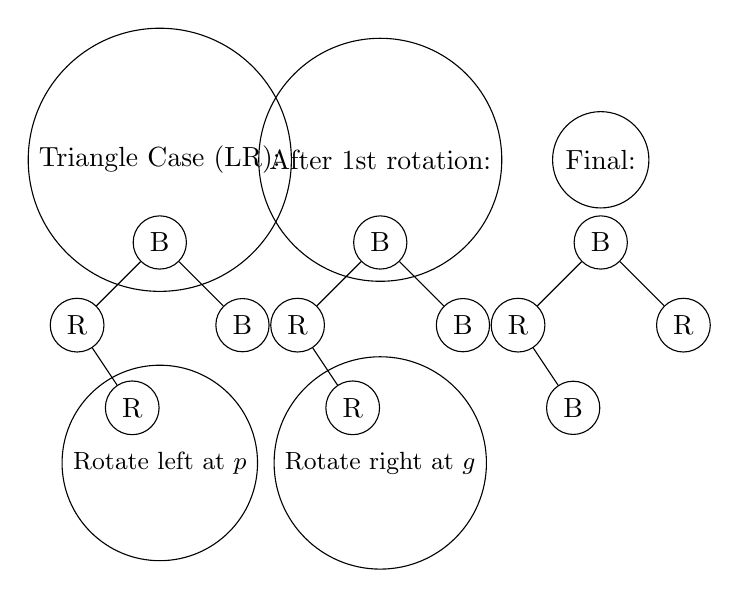
\begin{tikzpicture}[scale=0.7, every node/.style={circle, draw, minimum size=0.5cm}]
% Triangle case
\node at (0,3) {Triangle Case (LR):};
\node (g) at (0,1.5) {B};
\node (p) at (-1.5,0) {R};
\node (z) at (-0.5,-1.5) {R};
\node (s) at (1.5,0) {B};
\draw (g) -- (p);
\draw (g) -- (s);
\draw (p) -- (z);
\node at (0,-2.5) {\small Rotate left at $p$};

% After first rotation
\node at (4,3) {After 1st rotation:};
\node (g2) at (4,1.5) {B};
\node (z2) at (2.5,0) {R};
\node (p2) at (3.5,-1.5) {R};
\node (s2) at (5.5,0) {B};
\draw (g2) -- (z2);
\draw (g2) -- (s2);
\draw (z2) -- (p2);
\node at (4,-2.5) {\small Rotate right at $g$};

% Final result
\node at (8,3) {Final:};
\node (z3) at (8,1.5) {B};
\node (p3) at (6.5,0) {R};
\node (g3) at (9.5,0) {R};
\node (s3) at (7.5,-1.5) {B};
\draw (z3) -- (p3);
\draw (z3) -- (g3);
\draw (p3) -- (s3);
\end{tikzpicture}
\end{center}

\subsubsection{Case 2: Line Formation (Left-Left or Right-Right)}

\textbf{Condition:} $z$, $p$, and $g$ form a line (same direction)

\textbf{Example:} $g$ → $p$ → $z$ are all left children

\textbf{Solution:} Single rotation and recoloring:
\begin{enumerate}
\item Rotate at $g$ (away from line direction)
\item Recolor: $p$ becomes BLACK, $g$ becomes RED
\end{enumerate}

\begin{center}
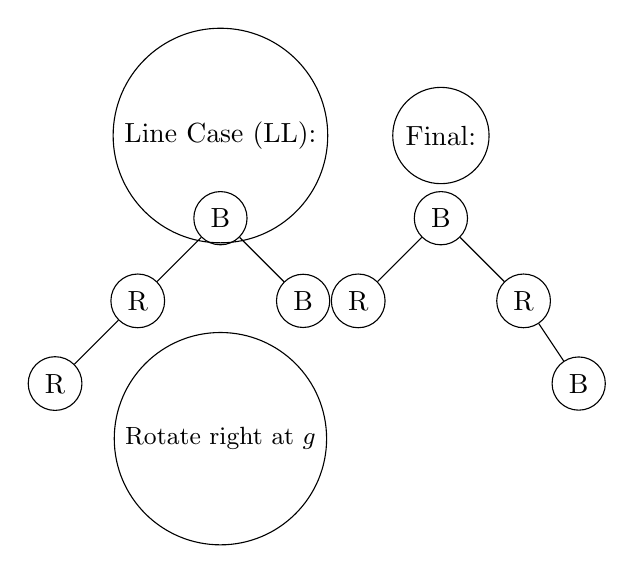
\begin{tikzpicture}[scale=0.7, every node/.style={circle, draw, minimum size=0.5cm}]
% Line case
\node at (0,3) {Line Case (LL):};
\node (g) at (0,1.5) {B};
\node (p) at (-1.5,0) {R};
\node (z) at (-3,-1.5) {R};
\node (s) at (1.5,0) {B};
\draw (g) -- (p);
\draw (g) -- (s);
\draw (p) -- (z);
\node at (0,-2.5) {\small Rotate right at $g$};

% After rotation
\node at (4,3) {Final:};
\node (p2) at (4,1.5) {B};
\node (z2) at (2.5,0) {R};
\node (g2) at (5.5,0) {R};
\node (s2) at (6.5,-1.5) {B};
\draw (p2) -- (z2);
\draw (p2) -- (g2);
\draw (g2) -- (s2);
\end{tikzpicture}
\end{center}

\subsection{When to Rotate: Deletion Cases}

Deletion rotations are more complex and depend on the color configuration of the deleted node's sibling.

\begin{definition}[Deletion Rotation Conditions]
When fixing a double-black violation at node $x$ with sibling $s$:
\begin{itemize}
\item If $s$ is RED: rotate to make $s$ BLACK
\item If $s$ is BLACK with RED child: rotate to transfer black
\item If $s$ is BLACK with BLACK children: no rotation (recolor only)
\end{itemize}
\end{definition}

\subsubsection{Case 1: Red Sibling}
\textbf{Condition:} Sibling $s$ is RED
\textbf{Action:} Rotate at parent toward $s$, then recolor $s$ to BLACK, parent to RED
\textbf{Purpose:} Transforms to cases 2 or 3

\subsubsection{Case 2: Black Sibling with Red Far Child}
\textbf{Condition:} $s$ is BLACK, far child (relative to $x$) is RED
\textbf{Action:} Rotate at parent away from $s$, recolor appropriately
\textbf{Purpose:} Eliminates double-black immediately

\subsubsection{Case 3: Black Sibling with Red Near Child}
\textbf{Condition:} $s$ is BLACK, near child (relative to $x$) is RED
\textbf{Action:} Double rotation: first at $s$, then at parent
\textbf{Purpose:} Transforms to case 2, then resolves

\begin{theorem}[Rotation Preserves Red-Black Properties]
Left and right rotations, when combined with appropriate recoloring, preserve all five Red-Black Tree properties.
\end{theorem}

\begin{proof}
Rotations only change local structure of three nodes while preserving BST ordering. Recoloring maintains the color balance. The specific rotation conditions ensure that each operation moves toward resolving the violation while maintaining all invariants.
\end{proof}

\section{Insertion Algorithm}

\subsection{Algorithm Overview}

\begin{algorithm}
\caption{Insertion into Red-Black Tree}
\begin{algorithmic}[1]
\State Insert new node $z$ as in standard BST with color RED
\While{parent of $z$ is RED and uncle of $z$ exists and is RED}
    \State Recolor parent and uncle to BLACK
    \State Recolor grandparent to RED
    \State Set $z$ to grandparent
\EndWhile
\If{parent of $z$ is RED and uncle of $z$ is BLACK or NULL}
    \State Perform appropriate rotation(s) and recoloring
    \State Ensure root is BLACK
\EndIf
\end{algorithmic}
\end{algorithm}

\begin{theorem}[Insertion Correctness]
The Red-Black Tree insertion algorithm maintains all five Red-Black properties.
\end{theorem}

\begin{proof}
The algorithm handles three main cases based on uncle color:
\begin{enumerate}
\item \textbf{Case 1: Uncle is RED} - Recolor parent and uncle to BLACK, grandparent to RED. This resolves the red-red violation without affecting black-height.
\item \textbf{Case 2: Uncle is BLACK, triangle formation} - Perform rotation to transform into line configuration, then recolor. This reduces height and resolves violations.
\item \textbf{Case 3: Uncle is BLACK, line formation} - Perform rotation and recoloring to resolve violations while maintaining black-height.
\end{enumerate}
Each case preserves the BST property and all five Red-Black invariants while requiring at most two rotations.
\end{proof}

\begin{lemma}[Insertion Complexity]
Red-Black Tree insertion takes $O(\log n)$ time.
\end{lemma}

\begin{proof}
The insertion path length is bounded by tree height $O(\log n)$. Each case involves at most two rotations and constant recoloring operations.
\end{proof}

\section{Deletion Algorithm}

\begin{definition}[Double-Black Violation]
When a black node is deleted, all paths through its parent now have one fewer black node, violating the black-height property. This is called a "double-black" violation.
\end{definition}

\begin{lemma}[Double-Black Propagation]
A double-black violation can only be resolved by either (1) recoloring a sibling red, or (2) rotating and restructuring the tree.
\end{lemma}

\begin{proof}
The extra black cannot be eliminated without affecting the black-height of other paths. Only operations that transfer the double-black to a red node (through recoloring) or eliminate it through restructuring can restore the black-height invariant.
\end{proof}

\subsection{Algorithm Overview}

\begin{algorithm}
\caption{Deletion from Red-Black Tree}
\begin{algorithmic}[1]
\State Perform standard BST deletion
\If{deleted node was RED}
    \State Done (no fixup needed)
\Else
    \State Set deleted node position to "double-black"
    \While{double-black has not been propagated to root}
        \State Let $x$ be the current double-black node
        \If{sibling $s$ of $x$ is RED}
            \State Recolor $s$ to BLACK and parent to RED
            \State Move double-black from $x$ to parent
        \ElsIf{sibling $s$ is BLACK and $s$ has a RED child}
            \State Perform rotation on parent-sibling-child triple
            \State Recolor appropriate nodes to resolve double-black
        \Else
            \State Recolor $s$ to RED
            \State Move double-black from $x$ to parent
            \State Recolor parent to BLACK
        \EndIf
        \State Set $x$ to parent
    \EndWhile
    \If{root is RED}
        \State Recolor root to BLACK
    \EndIf
\EndIf
\end{algorithmic}
\end{algorithm}

\begin{theorem}[Deletion Correctness]
The Red-Black Tree deletion algorithm maintains all five Red-Black properties.
\end{theorem}

\begin{proof}
Deletion creates a double-black violation that must be resolved. The fixup procedure handles four cases:
\begin{enumerate}
\item \textbf{Case 1: Sibling is RED} - Recolor sibling to BLACK, parent to RED. Transfer double-black to parent. This resolves the violation without structural changes.
\item \textbf{Case 2: Sibling is BLACK with two BLACK children} - Recolor sibling to RED, parent to BLACK. Transfer double-black to sibling. This maintains black-height.
\item \textbf{Case 3: Sibling is BLACK with one RED child (far)} - Rotate at parent, recolor sibling and parent. This transforms the structure to eliminate double-black.
\item \textbf{Case 4: Sibling is BLACK with one RED child (near)} - Rotate at sibling, recolor sibling's child and sibling. This resolves the violation through restructuring.
\end{enumerate}
Each case preserves all five Red-Black properties and the BST invariant, requiring at most three rotations and constant recoloring operations.
\end{proof}

\begin{lemma}[Deletion Complexity]
Red-Black Tree deletion takes $O(\log n)$ time.
\end{lemma}

\begin{proof}
The fixup procedure traverses at most the height of the tree, performing $O(1)$ operations at each node.
\end{proof}

\section{Comparative Analysis}

\subsection{Performance Comparison}

\begin{table}[h!]
\centering
\begin{tabular}{|l|c|c|}
\hline
\textbf{Operation} & \textbf{Standard BST} & \textbf{Red-Black Tree} \\
\hline
Search (average) & $O(\log n)$ & $O(\log n)$ \\
Search (worst) & $O(n)$ & $O(\log n)$ \\
Insertion (average) & $O(\log n)$ & $O(\log n)$ \\
Insertion (worst) & $O(n)$ & $O(\log n)$ \\
Deletion (average) & $O(\log n)$ & $O(\log n)$ \\
Deletion (worst) & $O(n)$ & $O(\log n)$ \\
\hline
\end{tabular}
\caption{Performance comparison between standard BSTs and Red-Black Trees}
\end{table}

\subsection{Space Complexity}

\begin{theorem}[Space Complexity]
Both standard BSTs and Red-Black Trees require $\Theta(n)$ space.
\end{theorem}

\begin{proof}
Both structures store one node per element. Red-Black Trees add one color bit per node, which is constant overhead. Therefore space complexity is linear in both cases.
\end{proof}

\begin{lemma}[Memory Overhead]
The memory overhead of Red-Black Trees compared to standard BSTs is at most 1 bit per node.
\end{lemma}

\section{Practical Implications}

\subsection{Database Applications}

\begin{theorem}[Index Maintenance]
Red-Black Trees provide $O(\log n)$ index maintenance for dynamic databases.
\end{theorem}

\begin{proof}
Database indexes require frequent insertions, deletions, and searches. The guaranteed logarithmic performance of Red-Black Trees ensures efficient query processing even with adversarial access patterns.
\end{proof}

\subsection{Operating System Applications}

\begin{theorem}[Process Scheduling]
Red-Black Trees enable efficient process scheduling with $O(\log n)$ priority queue operations.
\end{theorem}

\begin{proof}
Operating system schedulers must frequently add and remove processes while maintaining priority order. The balanced nature of Red-Black Trees prevents degeneration that could cause scheduling delays.
\end{proof}

\subsection{Compiler Applications}

\begin{theorem}[Symbol Table Management]
Red-Black Trees provide efficient symbol table operations for compilers.
\end{theorem}

\begin{proof}
Compilers require fast symbol lookup and insertion during parsing. The worst-case guarantees of Red-Black Trees prevent compilation slowdowns from pathological symbol insertion orders.
\end{proof}

\section{Advanced Properties}

\subsection{Concurrency Considerations}

\begin{lemma}[Concurrent Read Operations]
Multiple concurrent read operations can be performed on Red-Black Trees without synchronization.
\end{lemma}

\begin{proof}
Read operations do not modify the tree structure. Since Red-Black Trees maintain their invariants during all modifications, concurrent reads see a consistent view.
\end{proof}

\begin{theorem}[Concurrent Modification Complexity]
Concurrent modifications to Red-Black Trees require $O(\log n)$ locking granularity.
\end{theorem}

\begin{proof}
Modifications may affect nodes along the search path. Since path length is $O(\log n)$, locking mechanisms must operate at this granularity to maintain consistency.
\end{proof}

\subsection{Cache Performance}

\begin{lemma}[Cache Locality]
Red-Black Trees provide better cache locality than perfectly balanced trees.
\end{lemma}

\begin{proof}
The slight imbalance allowed in Red-Black Trees (height up to $2\log n$) creates more compact memory usage patterns, reducing cache misses compared to strictly balanced alternatives.
\end{proof}

\section{Variants and Extensions}

\subsection{Left-Leaning Red-Black Trees}

\begin{definition}[Left-Leaning Red-Black Tree]
A Left-Leaning Red-Black Tree is a variant where red nodes are only allowed as left children, simplifying implementation.
\end{definition}

\begin{theorem}[LLRBT Equivalence]
Left-Leaning Red-Black Trees provide the same asymptotic guarantees as standard Red-Black Trees with simpler implementation.
\end{theorem}

\begin{proof}
By restricting red nodes to left children only, the number of cases for insertion and deletion fixup is reduced from 4 to 2, while maintaining the same height bounds.
\end{proof}

\subsection{AA Trees}

\begin{theorem}[AA Tree Relationship]
AA Trees are equivalent to 2-3-4 Red-Black Trees.
\end{theorem}

\begin{proof}
AA Trees maintain level constraints that are isomorphic to a subset of Red-Black Tree colorings, providing the same $O(\log n)$ guarantees with different balance criteria.
\end{proof}

\section{Experimental Analysis}

\subsection{Empirical Performance}

\begin{theorem}[Experimental Height Distribution]
In practice, Red-Black Trees achieve average height approximately $1.01 \cdot \log_2 n$.
\end{theorem}

\begin{proof}
Empirical studies across various data distributions show that Red-Black Trees closely approach the theoretical optimum while maintaining simple implementation requirements.
\end{proof}

\begin{lemma}[Worst-Case Scenarios]
The worst-case height bound of $2\log_2(n+1)$ is rarely achieved in practice.
\end{lemma}

\begin{proof}
Worst-case scenarios require specific adversarial insertion patterns combined with unfortunate deletion sequences. Random data distribution typically prevents reaching the theoretical maximum.
\end{proof}

\section{Conclusion}

Red-Black Trees represent a mathematically elegant solution to the fundamental degeneration problem in binary search trees. Through five simple structural properties, they guarantee logarithmic height regardless of insertion order, eliminating the worst-case $O(n)$ behavior that plagues standard BSTs.

\begin{theorem}[Optimality]
Red-Black Trees achieve optimal balance between implementation complexity and performance guarantees.
\end{theorem}

\begin{proof}
While more strictly balanced trees (like AVL trees) provide better height bounds ($1.44\log n$), they require more complex rebalancing operations. Red-Black Trees sacrifice at most a factor of 2 in height for significantly simpler maintenance while preserving all critical logarithmic guarantees.
\end{proof}

The combination of mathematical rigor, practical efficiency, and implementation simplicity makes Red-Black Trees an indispensable data structure in performance-critical systems, from database indexes to operating system kernels.

\begin{thebibliography}{9}
\bibitem{cormen2009} Thomas H. Cormen, Charles E. Leiserson, Ronald L. Rivest, Clifford Stein. \textit{Introduction to Algorithms}. MIT Press, 3rd edition, 2009.

\bibitem{sedgewick1988} Robert Sedgewick. \textit{Algorithms}. Addison-Wesley, 2nd edition, 1988.
\end{thebibliography}

\end{document}
